\clearpage

\section{Comparing the Results}
\label{sec:comparing}

In this section, we will be comparing the results obtained by both the Theoretical Analysis and the Simulation.

\subsection{Results for the System at \textit{t $<$ 0}}

In the following tables, we can observe the results already presented in previous sections now side by side, with the first
2 tables being part of the Theoretical Analysis and the 3rd one being part of the Simulation. These are displayed in this
way as a means of easier representation.

\begin{table}[htb!]
  \begin{tabular}{|l|r|}
      \hline    
      {\bf Name} & {\bf Currents [A]} \\ \hline
      I1 & 2.3690260e-04\\\hline I2 & -2.4828279e-04\\\hline I3 & -1.1380187e-05\\\hline I4 & 1.2106395e-03\\\hline I5 & -2.4828279e-04\\\hline I6 & 9.7373690e-04\\\hline I7 & 9.7373690e-04\\\hline Ib & -2.4828279e-04\\\hline Id & 9.7373690e-04\\\hline Id & 0.0000000e+00\\\hline 
  \end{tabular}
\quad
  \begin{tabular}{|l|r|}
    \hline    
    {\bf Name} & {\bf Voltages [V]} \\ \hline
    \input{../mat/t2-t1-voltages.tex}
  \end{tabular}
\quad
  \begin{tabular}{|l|r|}
    \hline    
    {\bf Name} & {\bf Value [A or V]} \\ \hline
    @gb[i] & -2.48283e-04\\ \hline
@id[current] & 1.031476e-03\\ \hline
@r1[i] & 2.369026e-04\\ \hline
@r2[i] & -2.48283e-04\\ \hline
@r3[i] & -1.13802e-05\\ \hline
@r4[i] & 1.210639e-03\\ \hline
@r5[i] & 1.279759e-03\\ \hline
@r6[i] & 9.737369e-04\\ \hline
@r7[i] & 9.737369e-04\\ \hline
v(1) & 8.139731e+00\\ \hline
v(2) & 7.896243e+00\\ \hline
v(3) & 7.380521e+00\\ \hline
v(4) & 2.954689e+00\\ \hline
v(5) & 7.931699e+00\\ \hline
v(6) & 1.180782e+01\\ \hline
v(7) & 9.781670e-01\\ \hline
v(8) & 2.954689e+00\\ \hline

  \end{tabular}
  \caption{Results for the Circuit at $t<0$}
\end{table}

\clearpage
\subsection{Time- and Frequency-Dependent Analysis}

Lastly, here are the graphs we obtained by analysing the system side by side, Figures \ref{fig:sbs1}, \ref{fig:sbs2} and \ref{fig:sbs3}. It is clear that all of them are identical, which leads us to conclude, once more, that the study was succsseful.

\begin{figure}[ht]
\centering
\begin{subfigure}{.5\textwidth}
  \centering
  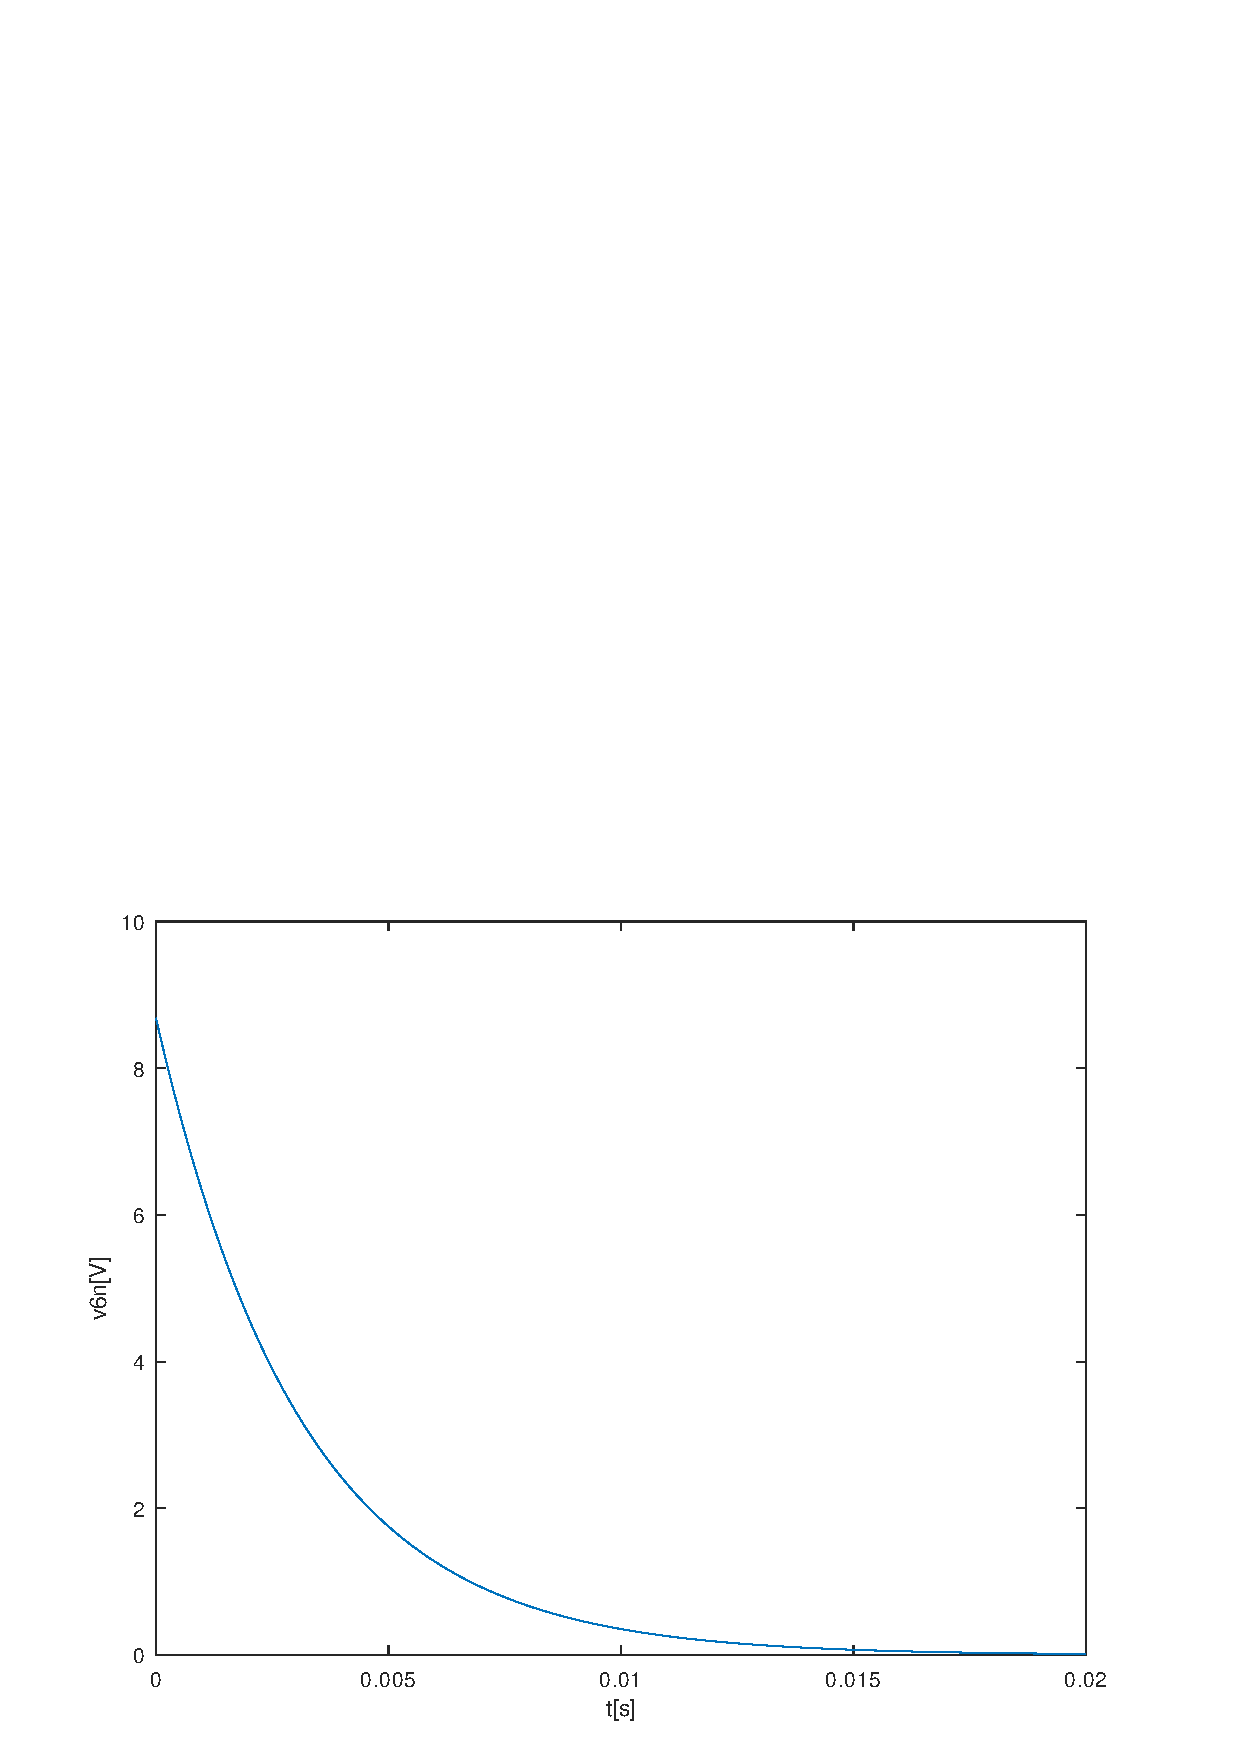
\includegraphics[width=.9\linewidth]{../mat/t2-t3.pdf}
\end{subfigure}%
\begin{subfigure}{.4\textwidth}
  \centering
  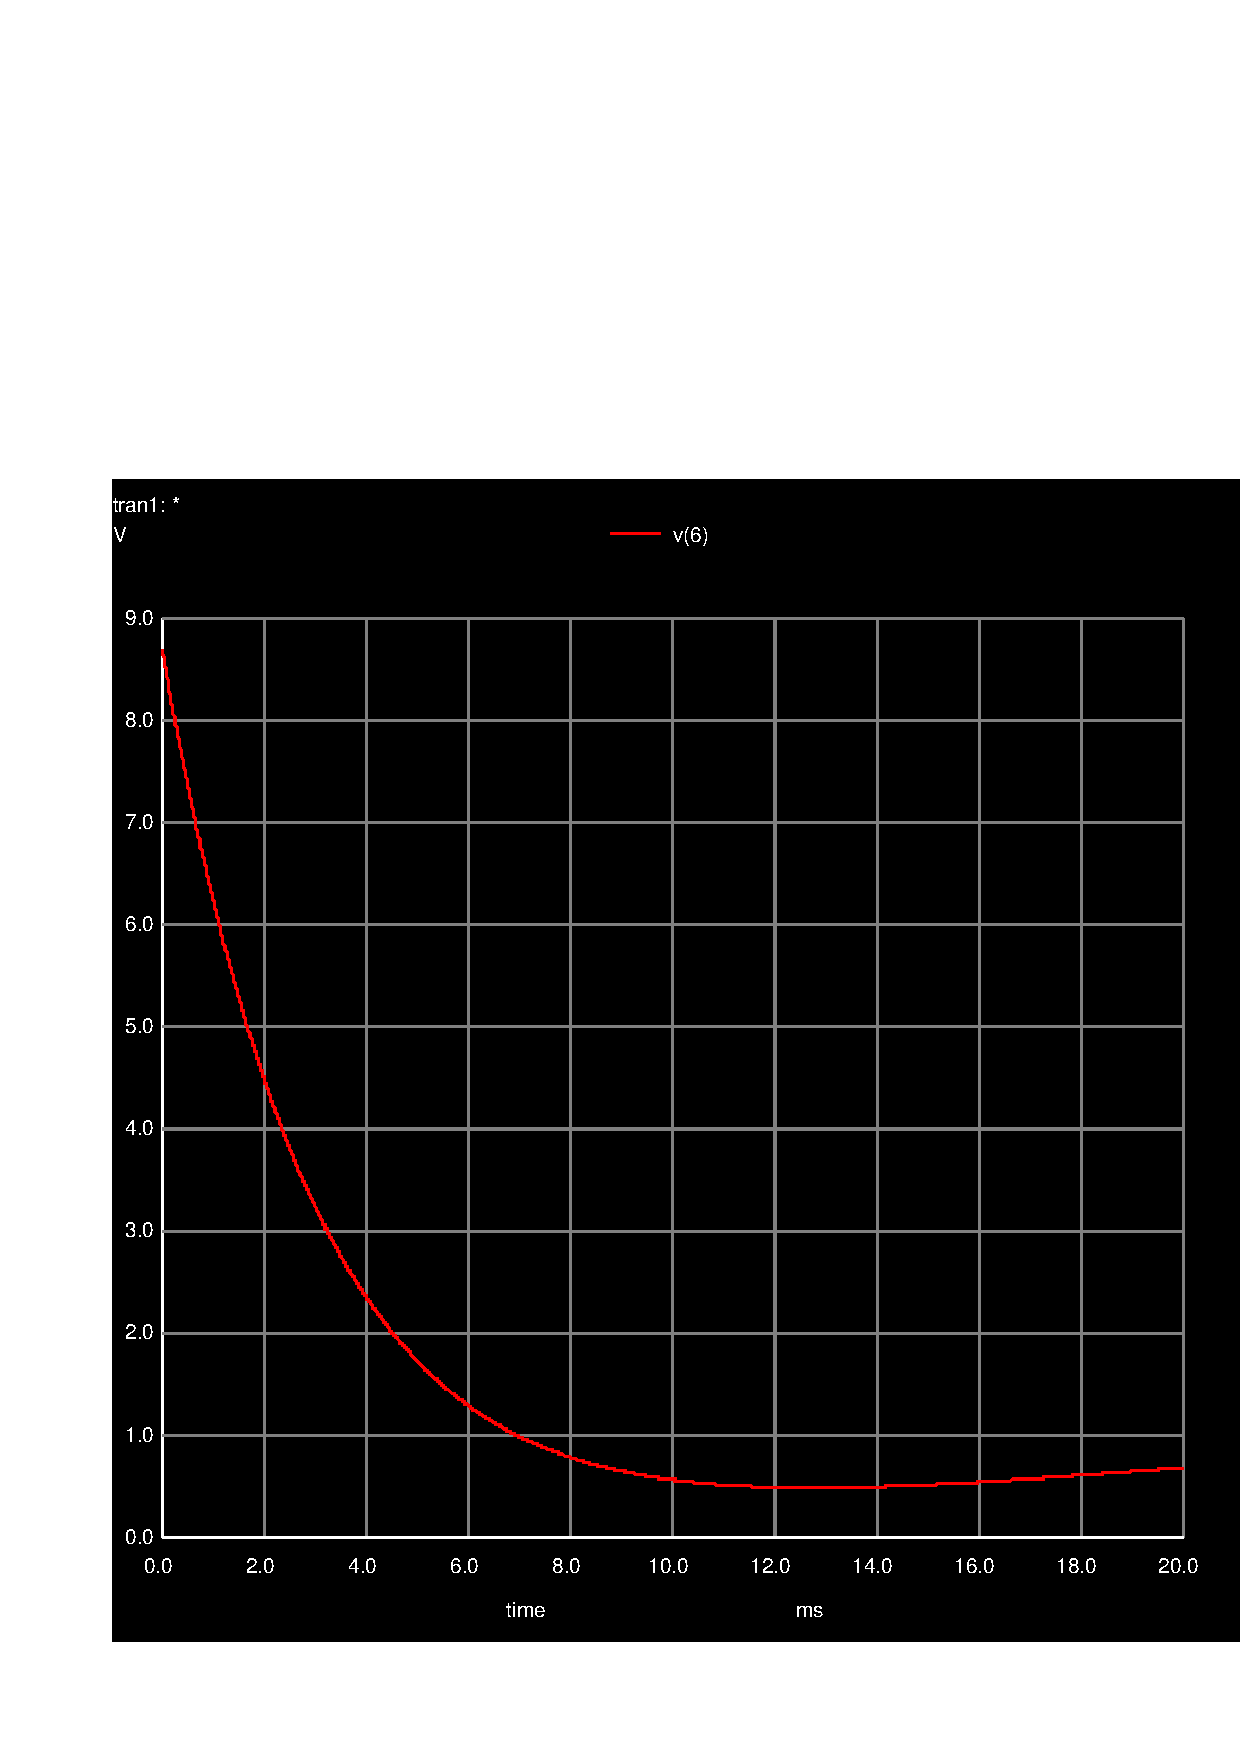
\includegraphics[width=.9\linewidth]{../sim/trans3.pdf}
\end{subfigure}
\caption{Results for f = 0Hz}
\label{fig:sbs1}
\end{figure}